\documentclass[a4paper]{article}
\usepackage[utf8]{inputenc}
\usepackage[spanish]{babel} 
\renewcommand{\spanishtablename}{Tabla} 
\spanishdecimal{.}
\usepackage{verbatim}
\usepackage{amssymb}
\usepackage{subcaption}
\usepackage{wrapfig}
\usepackage{graphicx}
\usepackage{hyperref}
\usepackage{mathtools}
\usepackage{float}
\usepackage{siunitx}
\renewcommand{\thefootnote}{\arabic{fotnote}}
\setlength{\parskip}{\baselineskip} 
\usepackage{pdfpages}

\begin{document}

\begin{titlepage}
\paragraph{}

\begin{center}
\vspace*{0.10in}
\begin{figure}
\raggedleft

\includegraphics[scale=0.12]{unam.png}
\hspace{7.2cm}
\raggedright
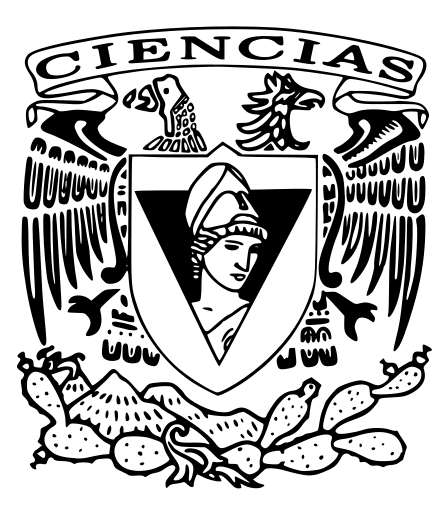
\includegraphics[scale=0.15]{fac.png}    
\end{figure}
\vspace*{0.5in}
UNIVERSIDAD NACIONAL AUTÓNOMA DE MÉXICO\\
\vspace*{0.2in}
FACULTAD DE CIENCIAS \\
\vspace*{0.5in}
\begin{large}
Laboratorio de Calor, Ondas y Fluidos\\
\end{large}
\vspace*{0.2in}
\begin{Large}
\textbf{Práctica 8} \\
\textbf{Tensión Superficial} \\
\end{Large}
\vspace*{0.3in}
\vspace*{0.3in}
\rule{80mm}{0.1mm}\\
\vspace*{0.1in}
\begin{large}
Profesor:  Quintanar Robles, Luis  \\
Ayudante: Quintanar Cortés, Luis Enrique \\
Mesa 1\\
Fecha de la práctica: 10 de octubre de 2019.\\
Alumnos: León Arenal Sebastian.\\
Robledo Ibarra Emiliano. \\
Toledo Castañeda, Akim Tarik.\\

\end{large}
\end{center}
\end{titlepage}

\section*{Resumen.}
Se calculó el coeficiente de tensión superficial de dos sustancias (glicerina y shampoo). Se obtuvieron los valores $(26\pm 5)\times10^{-3}  \frac{N}{m}$ para el shampoo y $45\pm 6)\times10^{-3}  \frac{N}{m}$ para la glicerina. De ello se concluyó que el método con el cual se trató con los datos requiere ser ajustado para no despreciar ciertos comportamientos del fluido que de hecho son importantes y que si se desprecian o idealizan, al operarlos reducen considerablemente los valores obtenidos, se propuso  formular correctamente un diámetro promedio que indique una tendencia y una nueva forma de aplicar la fuerza. Aunque se encontraron valores que relacionan a la fuerza y el radio, aún es posible mejorar dichos valores modificando ciertos aspectos del experimento.

\section*{Introducción.}
Con frecuencia podemos observar a las hojas o a los insectos "flotar" sobre la superficie de un cuerpo de agua. No se hallan sumergidos, por lo tanto no reciben el empuje según enuncia el principio de Arquímedes. En este caso el objeto está en la superficie por completo y nada de él se halla sumergido. [1]. Aquello que genera este fenómeno se le conoce como tensión superficial que se produce gracias a la fuerza de cohesión entre las moléculas que puede modificarse químicamente y parece que la superficie se "estira" lo cual  ejerce una fuerza de restitución en equilibrio con el peso del objeto. La tensión superficial $\gamma$ se define como la fuerza superficial
F por unidad de longitud L sobre la cual actúa: [1]

\begin{equation}
    \gamma = \frac{F}{L}
\end{equation}

El objetivo de este experimento fue medir la tensión superficial del shampoo y la glicerina por medio de dos variables: fuerza y la longitud para poder obtener la tensión superficial por medio de una razón; para ello se adecuó la fórmula a utilizar: como no se está hablando de condiciones ideales se consideran dos capas de líquido, además de que se consideraron a la misma altura y que por tanto conservaron las medidas del anillo utilizado (considerado circular), para las capas se idealizó su forma aproximada a la forma de un cilindro. Es así como la fórmula con la cual se relacionaron ambas cantidades medidas fue:

\begin{equation}
    \gamma = \frac{F}{\pi (d_i + d_f)}
\end{equation}

Donde $F$ representa la fuerza aplicada para levantar la columna, $d_i$ y $d_f$ los radios del anillo, $\pi$ la constante para calcular el perimetro de cada columna.

\section*{Procedimiento.}
Se llenó a la mitad una caja de petri con shampoo. Se colocó la caja de petri sobre una base de altura variable. Con  un soporte universal, una nuez y una pinza de tres dedos se construyó un soporte para colgar un dinamómetro y de él, un anillo de plástico atado con alambres para sumergirlo en el líquido; para poder medir la fuerza aplicada se colocó el cero del dinamómetro una vez colgado el aro. Es necesario asegurar que la base esté bien nivelada y que el anillo plástico esté paralelo a la superficie del líquido. Para nivelar la base de altura variable se ocupó un nivel; el anillo plástico se niveló empíricamente.

\begin{figure}[H]
    \centering
    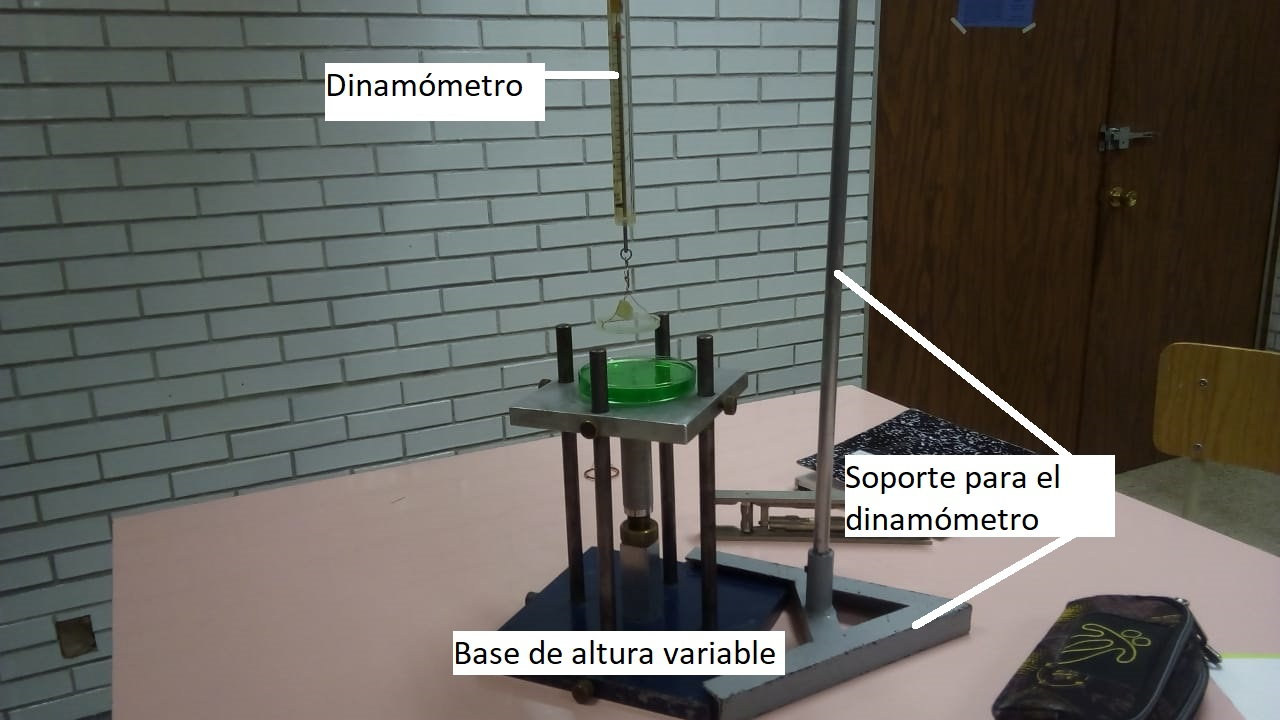
\includegraphics[width=10cm]{SistemaT-S.jpg}
    \caption{Sistema}
\end{figure}
 
 \begin{figure}[H]
    \centering
    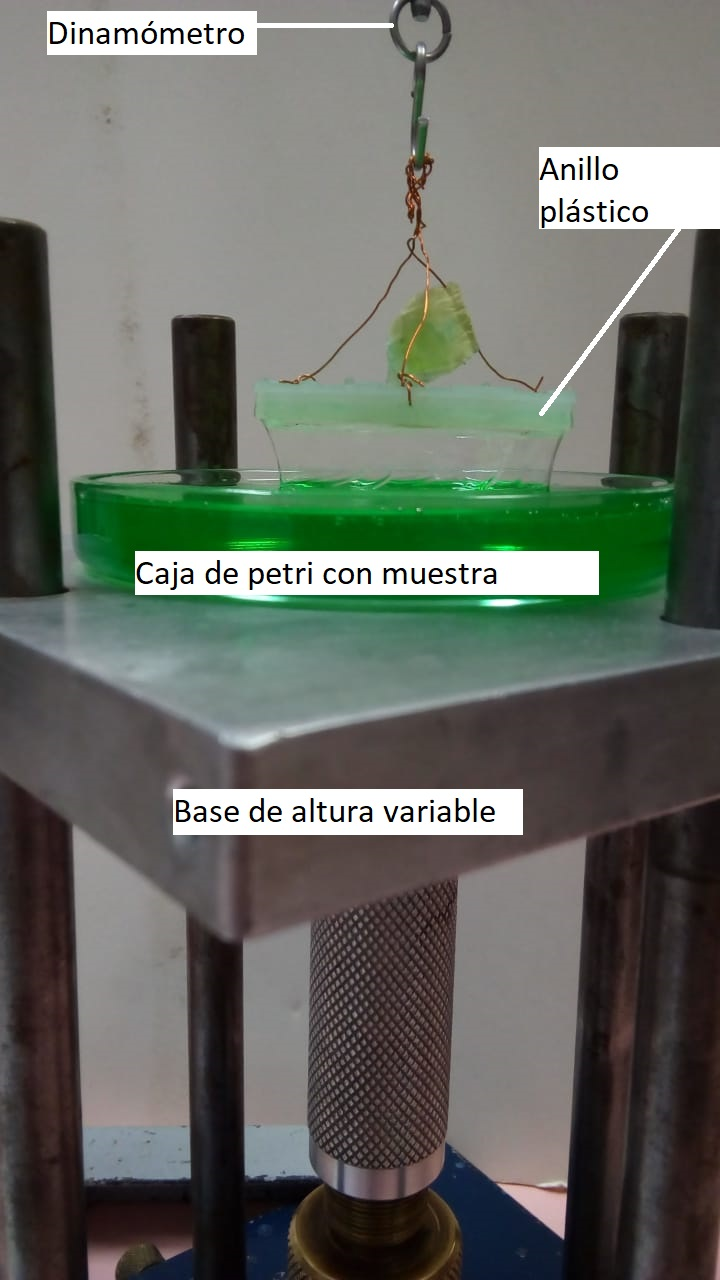
\includegraphics[width=10cm]{S-TS-Zoom.jpg}
    \caption{Vista cercana del sistema}
\end{figure}
 

Se alinearon la caja de petri y el anillo de plástico. Utilizando la base de altura variable, se pusieron en contacto el anillo plástico y el líquido. En esta parte del procedimiento es importante que el anillo plástico no esté sumergido en la glicerina para evitar la fuerza de empuje; el anillo debe tener su base completamente en contacto con la glicerina y no más. Con cuidado y para no perturbar el sistema, se fue bajando la altura de la base poco a poco. Se observa la formación de un cilindro de glicerina entre el anillo y la superficie de la glicerina en la caja de petri; conforme se separan la caja de petri del anillo se hace mas largo el cilindro hasta que éste se "rompe". Se registraron la diferencia de alturas y pesos en cuanto se observó la ruptura Se repitió el procedimiento para la glicerina. En total se registraron cinco mediciones del shampoo y cuatro para la glicerina.

Una vez medidos se operó con ellos, para cada apartado se obtuvo un valor promedio por líquido, que fue el ocupado para la obtención de la tensión superficial y se le otorgó la incertidumbre promedio, además de ello se realizaron las conversiones propias de unidades para el SI y se reportaron los valores de la tensión superficial con su incertidumbre propagada.

En cuanto a mediciones refiere, se realizó la decisión de sólo ocupar un aro de plástico por lo que se midieron sus radios interno y externo que, además, se consideraron como circunferencias perfectas; se registraron como $d_{int}$ al diámetro interior y $d_{ext}$ al exterior y debido a que ambos se midieron con un vernier se les otorgó incertidumbre de $0.002 cm$. Debido a que la plataforma se colocó una altura inicial $h_i$ y $h_f$ una altura final  superiores a la escala del vernier, se utilizó un flexómetro con incertidumbre de $0.05 cm$. Para la parte de la fuerza se contó con un dinamómetro de resolución $0.002 N$ que por tanto se le asignó incertidumbre de $0.001 N$.

\section*{Resultados.}
Aquí se colocan los datos obtenidos del shampoo y la glicerina, primero los diámetros del aro.

\begin{itemize}
    \item Diámetro interno:  $d_{int} = 4.875\pm0.002$ cm.
    \item Diámetro externo: $d_{ext} = 4.975\pm0.002$ cm.
\end{itemize}

\subsubsection*{Shampoo}
\begin{table}[H]
  \centering
    \begin{tabular}{|c|c|c|c|} \hline
    Medición & Altura inicial $h_i$ [cm] & Altura final $h_f$ [cm] & Fuerza [N] \\ \hline
    1     & $21.10\pm0.05$ & $20.10\pm0.05$ & $0.008\pm0.001$ \\ \hline
    2     & $20.90\pm0.05$ & $19.80\pm0.05$ & $0.008\pm0.001$ \\ \hline
    3     & $21.20\pm0.05$ & $20.20\pm0.05$ & $0.006\pm0.001$ \\ \hline
    4     & $21.00\pm0.05$ & $20.20\pm0.05$ & $0.008\pm0.001$ \\ \hline
    5     & $21.00\pm0.05$ & $20.20\pm0.05$ & $0.008\pm0.001$ \\ \hline
    \end{tabular}%
  \caption{Resultado de cinco mediciones para el shampoo, datos obtenidos directamente.}
\end{table}%

Para el shampoo se obtuvieron los datos promedio:
\begin{itemize}
    \item Diámetro interno: $d_{int} = 4.875\pm0.002$ cm.
    \item Diámetro externo: $d_{ext} = 4.975\pm0.002$ cm.
    \item Fuerza promedio: $\Delta F = 0.008\pm0.001$ N.
    \item Diferencia de altura: $\Delta h = 0.9\pm 0.1$ cm.
\end{itemize}

Y al utilizar los datos obtenidos de las mediciones se obtiene:
$$\gamma = (26\pm 5)\times10^{-3}  \frac{N}{m}$$

\subsubsection*{Glicerina}
\begin{table}[H]
  \centering
    \begin{tabular}{|c|c|c|c|} \hline
    Medición & Altura inicial $h_i$ [cm] & Altura final $h_f$ [cm] & Fuerza [N] \\ \hline
    1     & $22.10\pm0.05$ & $21.20\pm0.05$ & $0.016\pm0.001$ \\ \hline
    2     & $21.70\pm0.05$ & $20.90\pm0.05$ & $0.014\pm0.001$ \\ \hline
    3     & $22.20\pm0.05$ & $21.20\pm0.05$ & $0.014\pm0.001$ \\ \hline
    4     & $22.10\pm0.05$ & $21.20\pm0.05$ & $0.014\pm0.001$ \\ \hline
    \end{tabular}%
  \caption{Resultado de cuatro mediciones para la glicerina, los datos obtenidos directamente.}
\end{table}%

Para la glicerina se obtuvieron los datos promedio:
\begin{itemize}
    \item Diámetro interno: $d_{int} = 4.875\pm0.002$ cm.
    \item Diámetro externo: $d_{ext} = 4.975\pm0.002$ cm.
    \item Fuerza promedio: $\Delta F = 0.014\pm0.001$ N.
    \item Diferencia de altura: $\Delta h = 0.9\pm0.1$ cm.
\end{itemize}

Y al utilizar los datos obtenidos de las mediciones se obtiene:
$$\gamma = (45\pm 6)\times10^{-3}  \frac{N}{m}$$

\section*{Conclusiones.}
Primero que nada podemos ver que en muchas de las mediciones se alcanza una diferencia de longitud ''límite'' por llamarlo de una manera, que tiende a cierto valor, en el caso del shampoo en $0.9\pm0.1 cm$ y la glicerina en $0.9\pm0.1 cm$. También notamos que mientras la longitud limite hace eso, la fuerza realiza un efecto similar donde la fuerza en el shampoo es $0.008\pm0.001 N$ y la glicerina en $0.014\pm0.001 N$. Esto nos habla de una reproducibilidad en condiciones similares ya que estas medidas se realizaron  tratando de recrear en la medida de lo posible, es claro que el aro o anillo forma una parte crucial del experimento pues del mismo donde se tira, es por ello que el primer factor a interponerse a la reproducibilidad es este objeto que, no obstante, no genera incertidumbres ni errores suficientemente grandes o notorios. También es preciso hablar de como un detalle a revisar siempre fue la fuerza boyante que afectaba al cuerpo al sumergirlo pero que al extraer el aro desaparecía. Sin embargo, ya fuera del líquido la fuerza marcada por dinamómetro se hacía menor conforme pasaba el tiempo y la altura, de forma que se obtuvo un efecto de adelgazamiento de las capas.

Bajo las medidas ocupadas y los resultados debidos a ellos se obtiene que el  coeficiente (al menos en el que fue posible comparar, glicerina) es más pequeño al esperado teóricamente y que además no se contempla ni siquiera en la incertidumbre, este es $(45\pm 6)\times10^{-3}  \frac{N}{m}$ contra el teórico de $59\times10^{-3} \frac{N}{m}$ [3] y como se realizó un proceso similar con el shampoo se cree que también este pueda ser más bajo al real ( que se obtuvo igual a $(26\pm 5)\times10^{-3}  \frac{N}{m}$), a pesar de ello podemos ver que no es lo suficientemente lejano a dicho valor, lo cual nos habla de un error en la medición o el tratamiento de la fuerza y área; nos dimos cuenta que al separar el anillo del líquido era posible observar no un cilindro como dicta la teoría o como se hipotetizó sino que la forma era similar a la de una exponencial rotada sobre su eje que disminuía su radio conforme el anillo se separaba más y más, de forma que al romperse la capa de líquido el área era distinta a la de un cilindro y por tanto mucho más difícil de estimar, es por ello que la hipótesis de una columna de líquido en forma de cilindro hizo que los resultados se volviesen más imprecisos; se cree que el sistema tendía a su estado de mínima energía lo cual podría explicar el por qué no permanecía la columna cilíndrica.

A pesar de los materiales rudimentarios utilizados en el experimento los resultados obtenidos muestran una aproximación no tan deficiente para los coeficientes; en el aspecto experimental es claro que la aproximación de una superficie cilíndrica afecta, es por ello que se hace eco en un cambio de longitud de forma que se pueda hacer el equivalente al diámetro promedio:  esto podría hacerse midiendo el primer diámetro obtenido y promediarlo con el segundo al momento de reventarse la capa, puesto que hablamos de coeficientes cuya primera cifra significativa son las centésimas requerimos un mejor diseño experimental, es por ello que se propone también aplicar una fuerza constante al contrario de una variable, ya que en el experimento se esperó hasta que rompiera o se estabilizara, de esta manera se cree que sea posible observar como no cambia considerablemente el radio y se cuenta con una fuerza no decreciente (ya que conforme se dejó correr el tiempo el fluido escurría por las paredes) y aunque un poco más difícil de estimar la fuerza final, sería posible solucionar eso grabando el medidor.


\begin{thebibliography}{a}
\bibitem{pradery} \textsc{Resnick, R., Halliday, D., Krane, K.} (2001). \textit{Física Vol. 1}. ($4^a$ ed). México. GRUPO PATRIA CULTURAL,

\bibitem{pradery} \textsc{Bevington P., Robinson D.} (1969). \textit{Data Reduction and Error Analysis for the Physical Sciences
}. ($3^a$ ed). México. Mc Graw Hill.

\bibitem{pradery} \textsc{INN} (2019). \textit{Tensión superficial en los líquidos.} [en linea]. Recuperado el 14 de octubre de 2019 en \url{http://www.sc.ehu.es/sbweb/fisica/fluidos/tension/introduccion/introduccion.htm}


\end{thebibliography}
\end{document}

